% !TeX root = ../main.tex
% !TeX root = ../main.tex
% Add the above to each chapter to make compiling the PDF easier in some editors.

\chapter{Fundamentals of TUMLive}\label{chapter:fundamentals}

\section{GoCast Lecture Streaming Service}

\subsection{Overview}

GoCast is a fully self-hosted platform for live-streaming and recording of lectures, in use at the \ac{TUM} as \href{https://tum.live}{TUM-Live}.
TUM-Live offers live and on-demand videos of lectures and events from \ac{TUM}'s \href{https://www.cit.tum.de/}{School of Computation and Technology}, mainly by the department of informatics and mathematics. 
Its main features include:

\begin{itemize}
    \item Fully automatic live-Streaming from Auditoriums based on lecture schedules as imported from CAMPUSonline (campus management system used at \ac{TUM}).
    \item Self-service interface for lecturers to schedule and manage their \ac{VOD}s and streams.
    \item Automated import of lecture schedules and enrollments from CAMPUSonline.
    \item Self-streaming via third party streaming software such as \href{https://obsproject.com/}{OBS}, \href{https://zoom.us}{Zoom}, etc.
    \item Automatic recording of live-streams.
    \item Manual \ac{VOD} uploads.
    \item Automatic post-processing of recordings.
    \begin{itemize}
        \item Detects silence in videos and makes them skip-able.
        \item Transcribes videos and makes them searchable.
        \item Generates thumbnails.
    \end{itemize}
    \item Moderated live chat for listeners to ask questions.
    \begin{itemize}
        \item Polls can be created by lecturers.
        \item Questions can be upvoted by listeners.
        \item Questions can be marked as answered or hidden.
        \item Optional moderation features for lecturers.
    \end{itemize}
\end{itemize}

\subsection{Current System Architecture}

At the core of the GoCast system, there is the main \ac{API} built on the \href{https://github.com/gin-gonic/gin}{Gin-Gonic} Framework and connected to a \href{https://mariadb.org/}{MariaDB} Database. Its main functionality is to manage users, courses, streams, pull events from CAMPUSonline and scheduling tasks. For user authentication, it uses the provided services of \ac{TUM}'s \ac{SSO} and \ac{LDAP} to allow users to authenticate themselves with their university credentials. 
Next, whenever a lecture is recorded or livestreamed, the video data is processed by a TUM-Live Worker which then transcodes and segments the video into MPEG-2 compressed video transport stream files. These segments are then copied to a shared storage using the VOD Service component so that they can then later be distributed by the Edge Server.

\begin{figure}[htpb]
    \centering
    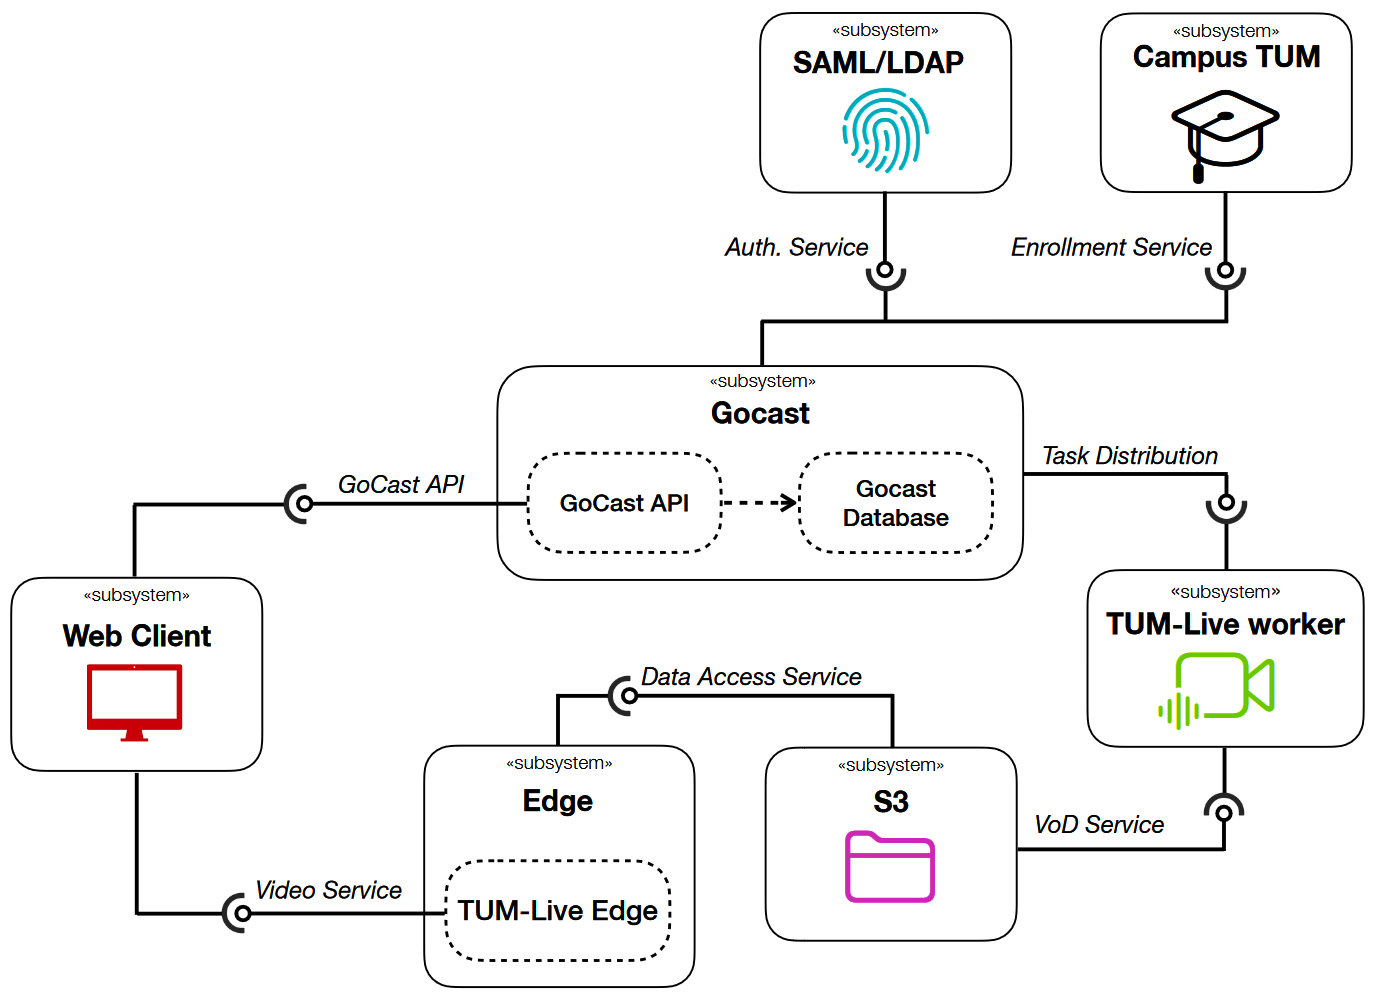
\includegraphics[width=420pt]{images/OldDeploymentDiagram2.png}
    \caption[Subsystem Decomposition]{Subsystem Decomposition Model of TUM-Live}\label{fig:old-system-architecture}
\end{figure}

\subsection{User Statistics of TUM-Live}\label{subsection:user-stats-tumlive}

Since its creation in February of 2021, GoCast has been used to stream thousands of hours of video every semester for more than 1300 courses, 20.000 streams and 30.000 students. The source code is open-source, accessible at \href{https://github.com/TUM-Dev/gocast}{github.com/TUM-Dev/gocast} and licensed under the MIT license.

\begin{figure}[htpb]
    \centering
    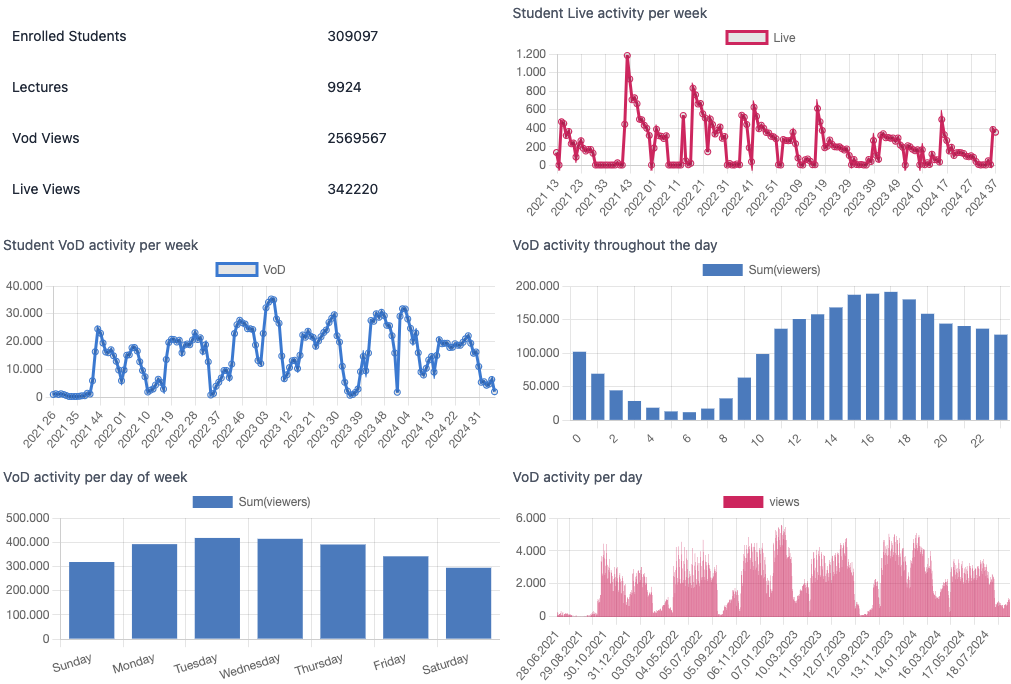
\includegraphics[width=\linewidth]{images/TUMLiveStats.png}
    \caption[TUMLive Statistics]{TUMLive Statistics}\label{fig:tumlive-stats}
\end{figure}
